% ======================== MODELO DE CASSANDRA ========================
\section{Modelo de Datos de Cassandra}
\label{sec:cassandra}

Cassandra es la capa de \textbf{series temporales y agregados}. El modelo sigue el principio de diseño orientado a consultas (\textit{query-first}): cada tabla existe para responder una pregunta concreta del \textit{dashboard} o de un indicador, y su clave de partición se elige para que esa pregunta se resuelva leyendo una sola partición. No hay \textit{joins}: cuando dos preguntas necesitan el mismo dato organizado de forma distinta, el dato se escribe dos veces. El esquema se crea con \repo{scripts/init_cassandra.cql}{scripts/init\_cassandra.cql}.

\subsection{Tablas}

El \textit{keyspace} \texttt{github\_metrics} contiene siete tablas (Tabla~\ref{tab:tablas-cassandra}).

\begin{table}[H]
\centering
\caption{Tablas de Cassandra: clave primaria y consulta que responde cada una. En la clave, la parte entre paréntesis dobles es la clave de partición y el resto son columnas de agrupamiento.}
\label{tab:tablas-cassandra}
\vspace{0.2cm}
\footnotesize
\begin{tabular}{@{}p{4.4cm}p{5.0cm}p{5.3cm}@{}}
\toprule
\textbf{Tabla} & \textbf{Clave primaria} & \textbf{Consulta que responde} \\
\midrule
\texttt{events\_by\_hour} &
\texttt{((event\_date)), event\_hour, event\_type} &
Eventos de cada tipo en cada hora de un día (Gráficos 1 y 2; KPI 1 y 2). \\
\addlinespace
\texttt{repo\_activity\_by\_day} &
\texttt{((event\_date)), repo\_name} &
Actividad de cada repositorio en un día, con conteos por tipo (Tabla de repositorios). \\
\addlinespace
\texttt{user\_activity\_by\_day} &
\texttt{((event\_date)), actor\_login} &
Eventos generados por cada usuario en un día (Tabla de usuarios; base del KPI 3). \\
\addlinespace
\texttt{user\_repo\_\bk{}interactions\_\bk{}by\_hour} &
\texttt{((event\_date, event\_hour)), actor\_login, repo\_name, event\_type} &
Qué hizo cada usuario sobre cada repositorio en una hora. Es la fuente de la etapa 5 (Neo4j). \\
\addlinespace
\texttt{daily\_totals} &
\texttt{((year)), event\_date} desc. &
Totales diarios de eventos, usuarios y repositorios distintos (Gráfico 3; KPI 3). \\
\addlinespace
\texttt{kpis\_by\_date} &
\texttt{((event\_date)), kpi\_name} &
Indicadores calculados por la etapa 6, leídos por el \textit{dashboard}. \\
\addlinespace
\texttt{pipeline\_runs} &
\texttt{((run\_date)), run\_hour} &
Trazabilidad e idempotencia: qué horas se procesaron y con cuántos eventos. \\
\bottomrule
\end{tabular}
\end{table}

\bloque{Definición de dos tablas representativas}
\begin{lstlisting}[style=cql]
-- Eventos de cada tipo en cada hora de un día.
-- Partición por día: las 24 horas de un día viven en una sola partición.
CREATE TABLE events_by_hour (
    event_date  date,
    event_hour  int,
    event_type  text,
    event_count int,
    PRIMARY KEY ((event_date), event_hour, event_type)
) WITH CLUSTERING ORDER BY (event_hour ASC, event_type ASC);

-- Totales diarios. Partición por año, días ordenados del más reciente al más antiguo.
CREATE TABLE daily_totals (
    year         int,
    event_date   date,
    total_events int,
    unique_users int,
    unique_repos int,
    PRIMARY KEY ((year), event_date)
) WITH CLUSTERING ORDER BY (event_date DESC);
\end{lstlisting}

\subsection{Decisiones de Particionamiento}

\begin{itemize}[leftmargin=*]
    \item \textbf{El día como clave de partición.} En \texttt{events\_by\_hour} una partición contiene a lo sumo $24 \times 16 = 384$ filas (horas por tipos de evento), por lo que su tamaño está acotado y no crece con el tiempo. El gráfico de eventos por hora se obtiene con una única lectura.
    \item \textbf{El año como clave de partición en \texttt{daily\_totals}.} La serie diaria completa se necesita siempre junta. Con el año como partición y la fecha como columna de agrupamiento descendente, la serie se lee en una sola consulta ya ordenada, y el día más reciente es la primera fila. La partición alcanza como máximo 366 filas.
    \item \textbf{Clave de partición compuesta (día, hora) en las interacciones.} Un día de octubre genera cientos de miles de pares usuario--repositorio; particionar solo por día produciría particiones demasiado grandes. Con (día, hora) cada partición corresponde exactamente a la unidad de trabajo del \textit{pipeline}, que la etapa 5 lee completa para construir el grafo.
    \item \textbf{Particiones anchas asumidas.} \texttt{repo\_activity\_by\_day} sí tiene particiones grandes en los días de mayor volumen (692 mil repositorios distintos el 12 de octubre). Se aceptó porque la consulta que la usa es un ranking del día, y el \textit{dashboard} limita la lectura histórica de esta tabla a los últimos siete días.
\end{itemize}

\subsection{Escritura e Idempotencia}

La etapa 4 (\repo{src/load_cassandra.py}{src/load\_cassandra.py}) lee de MongoDB los eventos de la hora, los agrega en memoria y los escribe con sentencias preparadas y 64 peticiones concurrentes. El tratamiento difiere según la granularidad de la tabla:

\begin{itemize}[leftmargin=*]
    \item Las tablas \textbf{por hora} (\texttt{events\_by\_hour}, interacciones) reciben un \texttt{INSERT} directo: la hora forma parte de la clave, de modo que reescribir una hora deja el mismo valor.
    \item Las tablas \textbf{por día} (repositorios y usuarios) deben reflejar las 24 corridas del día, pero no acumulan de una corrida a otra: para los repositorios y usuarios presentes en la hora, la etapa recalcula en MongoDB el total del día (una agregación \texttt{\$group} sobre el índice de \texttt{created\_at}) y escribe ese valor absoluto.
    \item \texttt{daily\_totals} se \textbf{recalcula} desde las tablas del día en cada corrida, por lo que es exacto y no arrastra errores de acumulación.
\end{itemize}

Como todas las escrituras son valores absolutos, la etapa es \textbf{idempotente por construcción}: repetir una hora, sea por un reintento de Airflow, por una escritura interrumpida a la mitad o por dos planificadores activos a la vez, deja el mismo resultado. La tabla \texttt{pipeline\_runs} sigue registrando las horas procesadas, y la etapa se omite si la hora ya figura en ella, pero ese registro solo evita rehacer el trabajo: ya no es lo que protege los conteos.

\paragraph{Cambio respecto de la primera versión.} Inicialmente las tablas diarias se actualizaban leyendo el valor existente, sumando y reescribiendo, y la idempotencia descansaba únicamente en \texttt{pipeline\_runs}. Ese esquema tenía una limitación identificada: si la escritura fallaba a mitad de una hora, antes de registrar la fila, el reintento podía acumular dos veces la parte ya escrita. El caso no llegó a observarse durante la operación, pero el recálculo desde MongoDB lo elimina. El cambio se validó el 14 de noviembre sobre los datos ya cargados: para cinco horas de días distintos, incluidos los de mayor volumen, el total recalculado coincidió con el valor acumulado en las 53,860 filas de repositorios y las 41,967 de usuarios comparadas, y reescribir dos veces una hora ya procesada (las 15:00 UTC del 12 de noviembre) dejó idénticas las cinco tablas. El costo es una lectura adicional de MongoDB por corrida: alrededor de un segundo en un día típico y unos 22 segundos en los días de mayor volumen, que superan el millón de eventos.

\subsection{Tamaño}

Al corte, \texttt{pipeline\_runs} tiene 1,056 filas (una por hora procesada), \texttt{events\_by\_hour} 14,933, \texttt{daily\_totals} 44 (una por día) y \texttt{kpis\_by\_date} 220 (cinco indicadores por día). El volumen Docker de Cassandra ocupa 1.7~GB. Según \texttt{nodetool tablestats}, el espacio vivo se concentra en tres tablas: \texttt{user\_repo\_\bk{}interactions\_\bk{}by\_hour} (973~MB), \texttt{repo\_activity\_by\_day} (467~MB) y \texttt{user\_activity\_by\_day} (181~MB). Las cuatro tablas que alimentan los gráficos temporales y los indicadores suman menos de 1~MB: el dato que el tablero lee con más frecuencia es también el más pequeño.

\subsection{Inspección Directa con Cassandra Web}

Las tablas se consultan también desde Cassandra Web, un explorador de solo lectura incluido en el \textit{stack} y accesible por túnel SSH. La Figura~\ref{fig:db-cassandra-web} muestra el espacio de claves \texttt{github\_metrics} con sus siete tablas y las filas de \texttt{daily\_totals}, que llegan ya ordenadas de la fecha más reciente a la más antigua por el orden de agrupamiento definido en la tabla.

\begin{figure}[H]
    \centering
    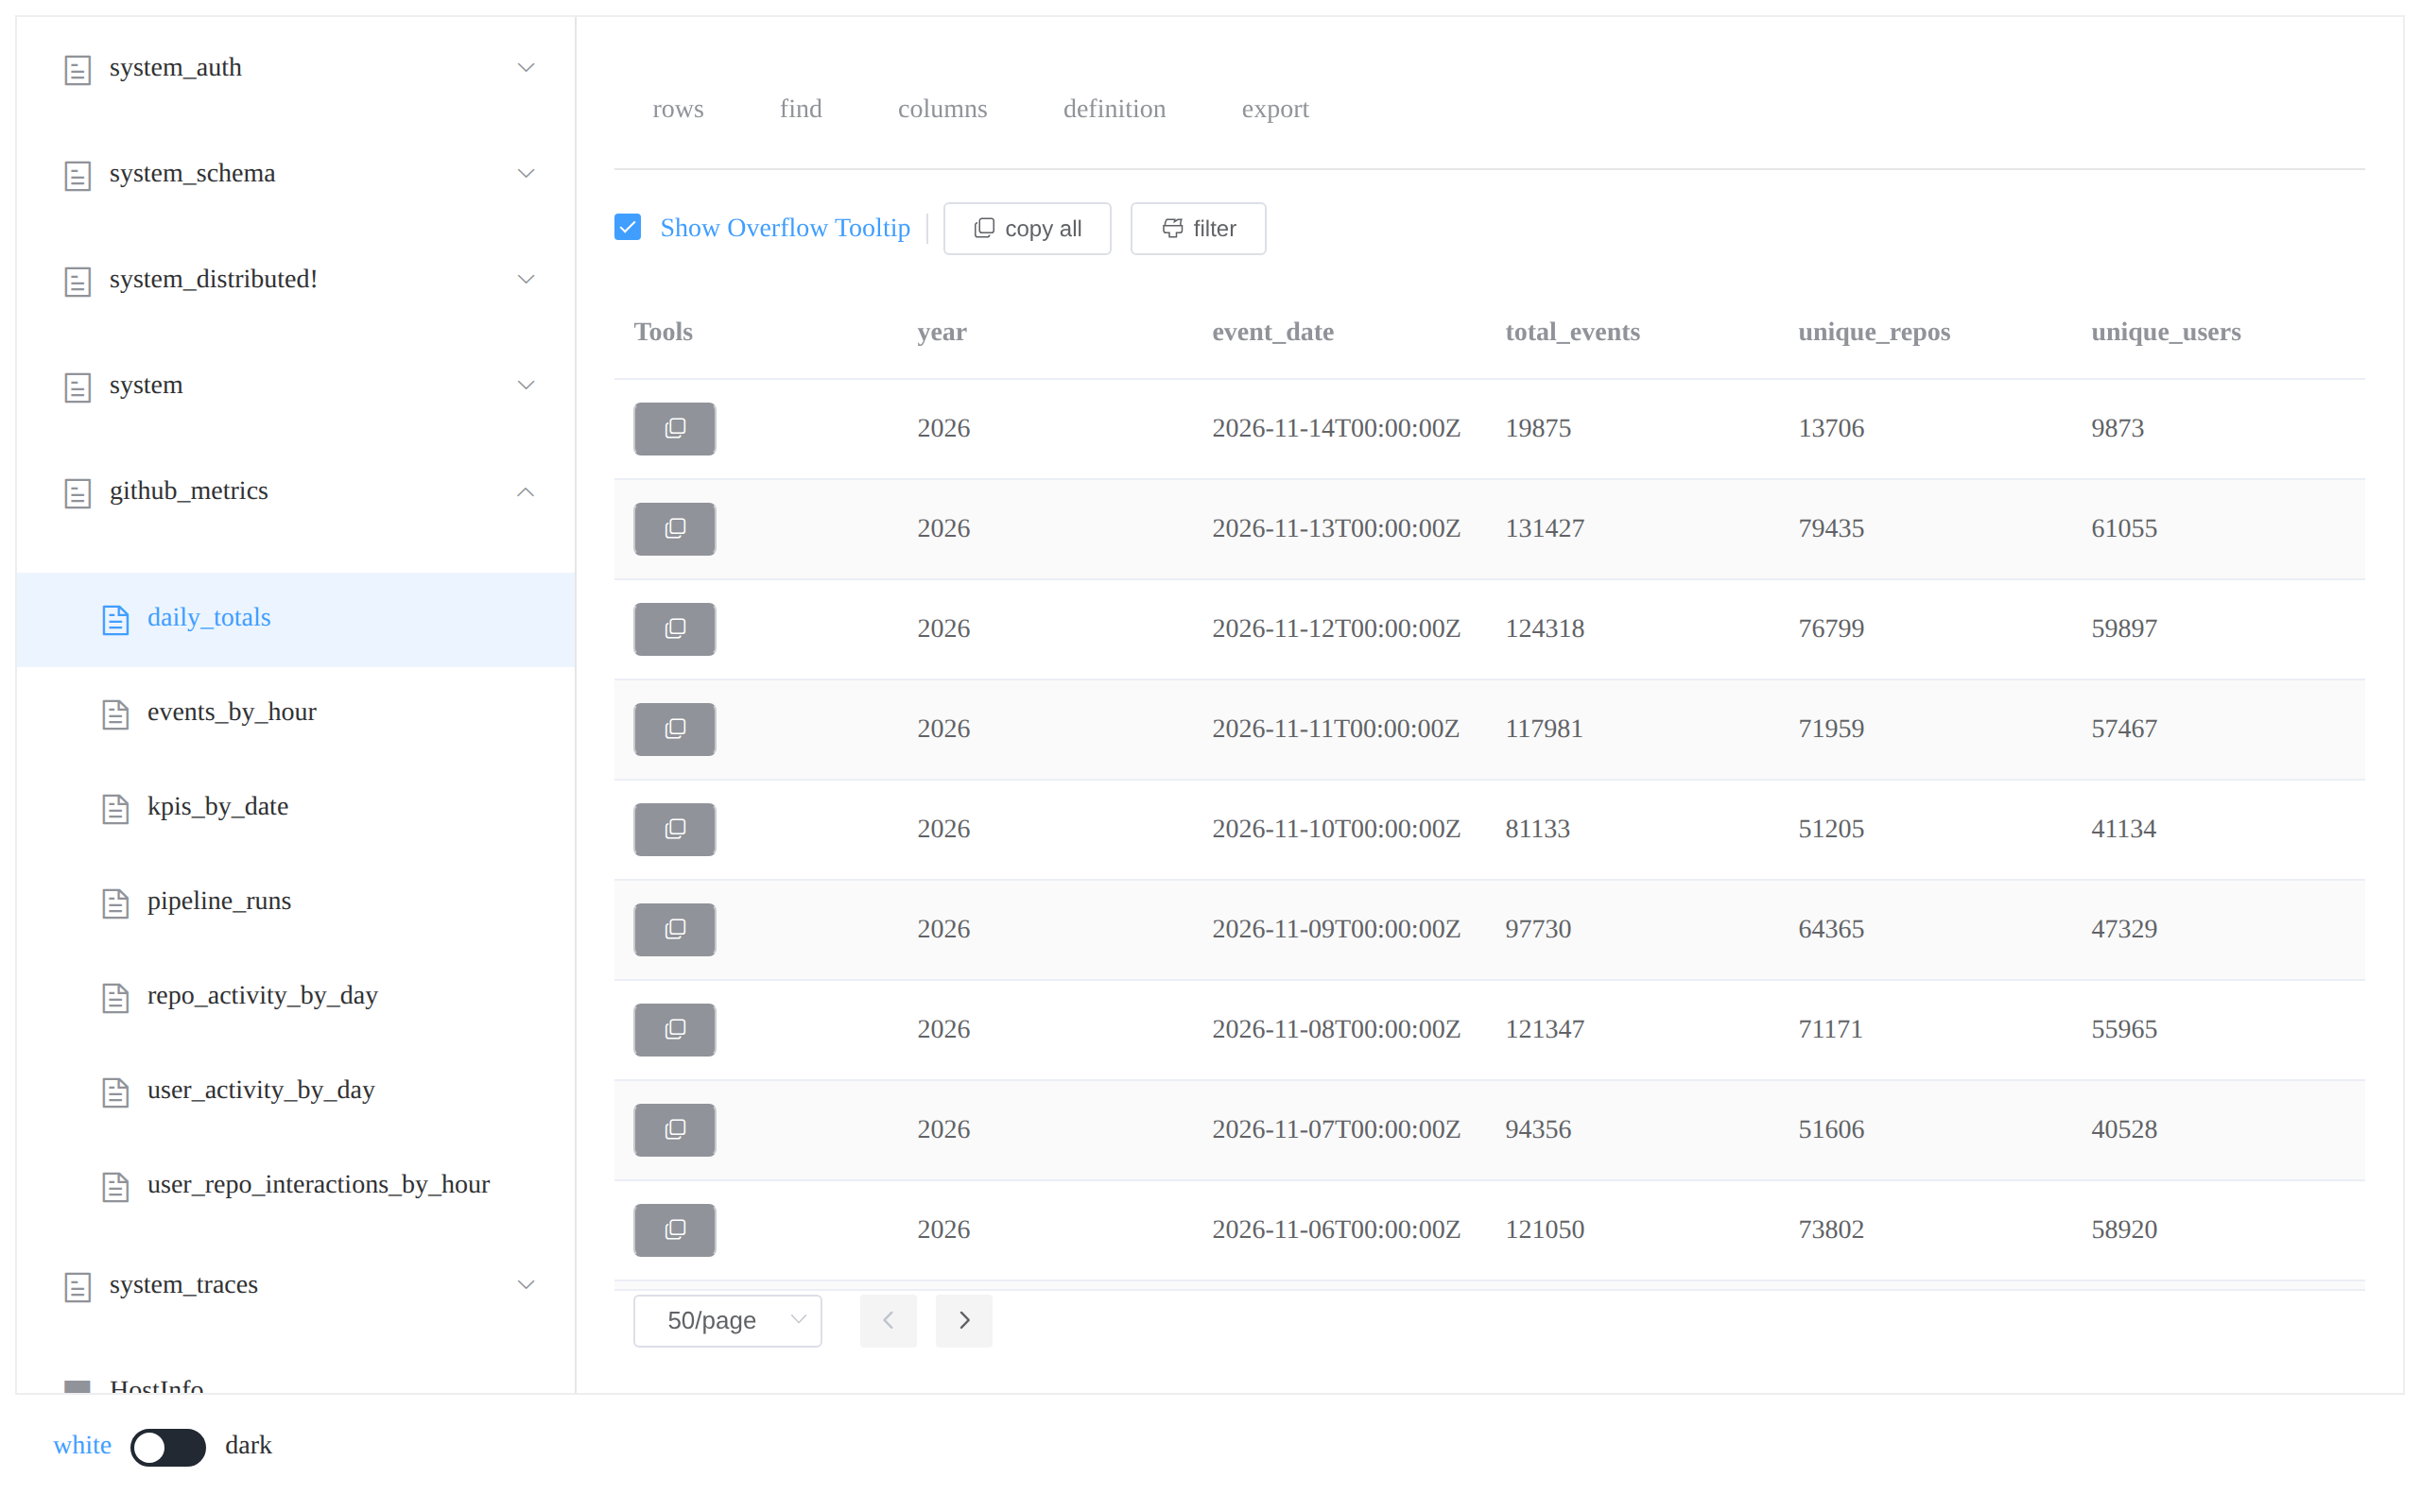
\includegraphics[width=0.93\textwidth]{db-cassandra-web.png}
    \caption{Tabla \texttt{daily\_totals} en Cassandra Web, capturada el 14 de noviembre. Cada fila resume un día: eventos, repositorios y usuarios distintos. La primera corresponde al día en curso, todavía parcial; las siguientes, a los últimos días completos del periodo.}
    \label{fig:db-cassandra-web}
\end{figure}
